\chapterimage{chapter_head_1.pdf}
\chapter{Espaces topologiques}

Dans ce chapitre, nous allons considérer plusieurs façons d'associer à un ensemble ce qu'on appelle un espace topologique.
\section{Filtres et voisinages}
\begin{definition}
    Soit $X\ne \varnothing$. Soit $\mathcal{F}\subseteq\partie(X)$ non vide. $\filtre$ est un filtre sur $X$ si $\filtre$ vérifie les propriétés suivantes
    
    \begin{enumerate}
        \item $\varnothing\notin\filtre$
        \item $\forall A,B\in \filtre \quad A\cap B\in \filtre$
        \item $\forall A\in \filtre,\forall B\in \partie(X) \quad (A\subseteq B)\Rightarrow(B\in \filtre)$
    \end{enumerate}
    
\end{definition}

\begin{remarque}
    Dans un filtre $\filtre$, on a toujours $X\in \filtre$ car $\filtre\neq\varnothing$. Il vient l'existence d'un $A\in \filtre$, d'où $X\in\filtre$ car $A\subseteq X\in\partie(X)$
\end{remarque}
\begin{notation}
    Soit $\varnothing\ne Y\subseteq X$. On note par $\filtre_Y := \{ Z\in\partie X\mid Y\subseteq Z\}$ le filtre engendré par $Y$. Il s'agit d'un filtre sur $X$
\end{notation}
\begin{proof}
    \begin{enumerate}
        \item Soit $A\in\filtre_Y$ Clairement, $A\ne \varnothing$, car sinon, on aurait $Y\subseteq \varnothing$ d'où $Y = \varnothing$.
        \item Clairement, si $Y\subseteq A,B\subseteq X$, on a $Y\subseteq A \cap B\subseteq X$.
        \item Si $Y\subseteq A\subseteq X$ et $B\subseteq X$, on a, par transitivité, $Y\subseteq B\subseteq X$.
    \end{enumerate}
\end{proof}
\begin{notation}
    Lorsque le contexte est clair (par exemple si il est certain que $\forall a\in X,\ \neg(a\subseteq X)$), on simplifie l'écriture de $\filtre_{\{a\}}$ en notant $\filtre_a$. 
\end{notation}
\begin{proposition}
Si $\mathscr{G}$ est un filtre étendant $\filtre_a$ \textit{i.e} $\mathscr G$ est un filtre tel que $\filtre_a \subseteq\mathscr{G}$ alors $\mathscr{G}=\filtre_a$.
\end{proposition}
\begin{proof}
En effet, pour $B\in \mathscr{G}$. Supposons par l'absurde que $a\notin B$. 
Alors $\{a\}\cap B = \varnothing$. 
Or $\{a\}\in\mathscr{G}$ et $B\in\mathscr{G}$, donc par stabilité des filtres par intersection finie, 
on aurait $\varnothing \in \mathscr{G}$, ce qui est absurde. 
Ainsi $a\in B$, donc $B\in \filtre_a$. 
On conclut que $\mathscr{G}\subseteq \filtre_a$. On dit que $\filtre_a$ est un filtre maximal.
\end{proof}

\begin{exemple}[Filtre de Frêchet]On appelle filtre de Frêchet, ou filtre des cofinis de $X$, le filtre $\{A\subseteq X \mid X\setminus A \text{ est fini}\}$
\end{exemple}

\begin{proposition}
    Soit $X\ne\varnothing$ un ensemble fini. Alors, l'ensemble des filtres sur $X$ est $\{\filtre_Y\mid Y\subseteq X\}$ 
\end{proposition}
\begin{proof}
    Clairement, les $\filtre_Y$ sont des filtres sur $X$. Réciproquement, soit $\filtre$ un filtre sur $X$. Alors, par définition des filtres, $\bigcap_{A\in\filtre}A\in\filtre$ car $\filtre\subseteq\partie(X)$ est fini. En effet, $X$ est fini, donc $\partie(X)$ l'est aussi. 
\end{proof}

\begin{definition}
    Soit $X\neq \varnothing$. On dit que $\voisinage:=\left(\voisinage_a\right)_{a\in X}$ est une famille (d'ensemble) de voisinages de points de $X$ si les propriétés suivantes sont vérifiées.    
    \begin{enumerate}
        \item $\forall a\in X, \voisinage_a$ est un filtre sur $X$
        \item $\forall a \in X,\forall V\in\voisinage_a, a\in V $
        \item  $\forall a\in X,\forall V\in \voisinage_a\text{ alors }\exists W\in \voisinage_a\quad W\subseteq V$ et $\forall w\in W,\; V\in \voisinage_w$ (cohérence)
    \end{enumerate}
\end{definition}
\begin{notation}
    Soient $a\in X, V\subseteq X,\voisinage$ une famille (d'ensembles) de voisinages. On dit que $V$ est un voisinage de $a$ si $V\in\voisinage_a$
\end{notation}
\begin{proposition}
De façon équivalente, on peut remplacer la cohérence par :
$$\forall a\in X,\forall V\in \voisinage_a, \exists W\in \voisinage_a , W\subseteq V, \forall w\in W, W\in \voisinage_w$$  
\end{proposition}
\begin{proof}
    Montrons l'équivalence :
    \begin{description}
    \item[($\si$) : ]Par extension, $W\in\voisinage_w$ implique $V\in\voisinage_w$.
        \item[($\alors$) : ]Soient $a\in X,V\in\voisinage_a$. Prenons $W'=\{x\in V\mid V\in\voisinage_x\}$. Remarquons qu'on a bien $W'\subseteq V$. Soit $x\in W'$. Par définition $V\in\voisinage_x$, on peut donc utiliser $3$ pour obtenir $W_y\in\voisinage_y$ tel que $W\subseteq V$ et $\forall w\in W_y,V\in \voisinage_y$ \textit{i.e.} $W_y\in\voisinage_y$ et $W_y\subseteq W'$. Donc $\forall y\in W',W'\in\voisinage_y$. En particulier, on a $W'\in\voisinage_a$ car $a\in W'$.
    \end{description}
\end{proof}
\begin{definition}
Un espace topologique est la donnée d'un ensemble $X$ non vide et d'une famille de voisinages $\voisinage$ sur $X$.
\end{definition}

\begin{definition}
On définit les deux concepts suivants :
\begin{itemize}
    \item Un ouvert de $(X,\voisinage)$ est un ensemble qui est un voisinage de tous ses points.
    \item Un fermé de $(X,\voisinage)$ est un ensemble dont le complémentaire est un ouvert.
\end{itemize}
\end{definition}

\begin{definition}
On définit les deux concepts suivants :
\begin{itemize}
    \item  L'adhérence de $A$, notée $\operatorname{adh}(A)$ ou encore $\overline{A}$, est le plus petit fermé $\ferme$  tel que $A\subseteq \ferme$.
    \item  L'intérieur de $A$, noté $\operatorname{int}(A)$, est le plus grand ouvert $\ouvert$ tel que $\ouvert\subseteq A$.
\end{itemize}   
\end{definition}

\begin{exemple}[Topologie discrète]
    Pour chaque $a \in X$, prenons $\voisinage_a=\filtre_a$. Montrons que ce choix du filtre $\filtre_a$ pour chaque point $a\in X$ vérifie l'axiome de cohérence.
\end{exemple}
\begin{proof}
    Soit $V\in \voisinage_a$, il faut trouver $W\in \voisinage_a$, $W\subseteq V$ tel que $V$ soit un voisinage de tous les points de $W$. On prend $W=\{a\}$ car $\{a\}\subseteq V$ et $\{a\}$ appartiennent à $\voisinage_a$. On peut aussi prendre $W=V$ car tous les voisinages sont ouverts pour la topologie discrète. On a que l'ensemble des ouverts pour la topologie discrète est $\partie(X)$.
\end{proof}
\section{Ouverts}
\begin{definition}
    Soit $\topologie\subseteq \partie(X)$. On dit que c'est une famille d'ouverts de $X$ ssi
    \begin{enumerate}
        \item $\varnothing,X\in \topologie$
        \item Si $(\ouvert_i)_{i\in I}$ est une famille d'éléments de $\topologie$ alors $\bigcup_{i\in I}\ouvert_i\in \topologie$
        \item Si $\ouvert_1$ et $\ouvert_2\in \topologie$, alors $\ouvert_1\cap \ouvert_2\in \topologie$ 
    \end{enumerate}
    Dans ce cas, on dira que $\topologie$ est une topologie.
\end{definition}
\begin{proposition}
    Une intersection quelconque de topologies est une topologie.
\end{proposition}
\begin{proof}
Soit $(\topologie_i)_{i\in I}$ une famille de topologies. Montrons que $\bigcap_{i\in I}\topologie_i$ est une topologie. Vérifions que les trois axiomes sont respectés.
\begin{enumerate}
    \item Comme pour tout $i\in I\quad \topologie_i$ est une topologie, on a $\varnothing, X\in \topologie_i$. Donc on a bien \[\varnothing,X\in \bigcap_{i\in I}\topologie_i\]
    \item Soit $(\ouvert_j)_{j\in J}$ une famille d'éléments de $\bigcap_{i\in I}\topologie_i$ alors montrons que
    \[\bigcup_{j\in J}\ouvert_j\in \bigcap_{i\in I}\topologie_i
    \]
    Cette appartenance est vraie puisque pour tout $j\in J \; \ouvert_j\in \bigcap_{i\in I}\topologie_i$ donc l'union appartient également à $\bigcap_{i\in I}\topologie_i$ car les $\topologie_i$ sont des topologies.
    \item Soit $\ouvert_1,\ouvert_2\in \bigcap_{i\in I}\topologie_i$, montrons que $\ouvert_1\cap\ouvert_2\in \bigcap_{i\in I}\topologie_i$. De même que au point 2), puisque $\ouvert_1$ et $\ouvert_2$ appartiennent tous deux à chacune des topologies $\topologie_i$, leur intersection appartiennent donc également à chacune des topologies et donc $\ouvert_1\cap\ouvert_2$ appartient bien à l'intersections des $\topologie_i$.
\end{enumerate}
\end{proof}
\begin{definition}
    On définit les deux applications suivantes:
    \begin{align*}
        \fonction{\mathscr{V}}{\{\text{ Topologie sur }X\}\to \{ \text{ Famille de voisinage sur } X\}}{ \topologie\mapsto (\voisinage_a)_{a\in X}\text{ avec }\voisinage_a := \{V\subseteq X\mid \exists \ouvert\in \topologie, a\in \ouvert\subseteq V\}}
    \end{align*}
    \begin{align*}
        \fonction{\mathscr{T}}{\{ \text{ Famille de voisinage sur } X\}\to\{\text{ Topologie sur }X\} }{ \voisinage\mapsto \{ \varnothing\}\cup\{V\in\partie(X)\mid \forall x\in\ouvert,\ \ouvert\in\voisinage_x\}}
    \end{align*}   
\end{definition}
Montrons que nos applications sont bien définies, càd que l'image de ces fonctions est bien incluse à leur ensemble d'arrivée respectif.
\begin{proof}
Montrons que nos applications sont bien définies :
    \begin{description}
        \item[Bonne définition de $\mathscr{V}$ :] 
        Soit $\topologie$ une topologie sur $X$. Montrons que $\{(\voisinage_a)_{a\in X}\mid \voisinage_a := \{V\subseteq X\mid \exists \ouvert\in \topologie, a\in \ouvert\subseteq V\}\}$ est une famille de voisinages. Commençons par montrer que $\forall a, \voisinage_a$ est un filtre. Vérifions chaque axiome des filtres :\begin{enumerate}
            \item D'abord, on a $\forall V\in\voisinage_a, a\in V$ par définition, d'où $\varnothing\not\in\voisinage_a$. 
            \item Soient $V_1,V_2\in\voisinage_a$. On veut montrer que $V_1\cap V_2\in\voisinage_a$. Par définition, il existe $\ouvert_1,\ouvert_2\in\topologie$ tels que $a\in\ouvert_1\subseteq V_1,a\in \ouvert_2\subseteq V_2$. On a alors $a\in\ouvert_1\cap\ouvert_2,\ouvert_1\cap\ouvert_2\in\topologie$ et $\ouvert_1\cap\ouvert_2\subseteq V_1\cap V_2$. Il vient $V_1\cap V_2\in\voisinage_a$.
            \item Montrons que $\voisinage_a$ est stable par extension. Soient $V\in\voisinage_a,W\in\partie(X)$. Supposons que $V\subseteq W$. Il vient l'existence de $\ouvert\in\topologie$ tel que $a\in\ouvert\subseteq V\subseteq W$, d'où $W\in\voisinage_a$.
        \end{enumerate}
        On a bien $\forall V\in\voisinage_a, a\in V$ par définition. Il reste à montrer la cohérence. Soit $V\in\voisinage_a$. Soit $\ouvert\in\topologie$ tel que $\ouvert \subseteq V$. Prenons $W=\ouvert$. Soit $w\in W$. On a bien $V\in\voisinage_w$ car $w\in W\subseteq V$.
        \item[Bonne définition de $\mathscr{T}$] Soit $\voisinage$ une famille de voisinages sur $X$. Montrons que $\{V\in\voisinage_a\mid a\in X, V \text{ est ouvert}\}$ est une topologie.
        \begin{enumerate}
            \item On a bien $\varnothing\in\mathscr T_\voisinage$ et $X\in\mathscr{T}_\voisinage$ car $\forall a \in X,X\in\voisinage_a$ par propriété des filtres.
            \item Soit $(\ouvert_i)_i\in I$ une famille d'éléments de $\mathscr{T}_\voisinage$. Montrons que $\bigcup_{i\in I}\ouvert_i\in\mathscr{T}_\voisinage$. Soit $x\in\bigcup_{i\in I}\ouvert_i$. Alors $\exists j\in I, x\in\ouvert_i$. Comme $\ouvert_j\subseteq\bigcup_{i\in I}\ouvert_i$ et que $\ouvert_j\in\voisinage_x$, on a que $\bigcup_{i\in I}\ouvert_i\in\voisinage_x$
            \item Soit $\ouvert_1,\ouvert_2\in\mathscr T_\voisinage$. Soit $x\in \ouvert_1\cap\ouvert_2$. Comme $\ouvert_1,\ouvert_2\in\voisinage_x$, par définition d'un filtre $\ouvert_1\cap\ouvert_2\in\voisinage_x$
        \end{enumerate}
    \end{description}
\end{proof}
\begin{proposition}
    $\mathscr{V}$ et $\mathscr{T}$ sont bijectives, et inverses l'une de l'autre.
\end{proposition}
\begin{proof}
\begin{itemize}
    \item Soit $\voisinage$ une famille de voisinages. Montrons que $\mathscr{V}(\mathscr{T}(\voisinage))=\voisinage$. Soit $a\in X$. On a $\voisinage_a = \{V\in\voisinage_a\}=\{V\in\voisinage_a\mid\exists\ouvert\in\voisinage_a,\ouvert\subseteq V,\ouvert\text{ est ouvert }\}$ par propriété des voisinage. Or, avec $\ouvert\in\partie(X)$, on a que $(\ouvert\in\voisinage_a,\ouvert\text{ est ouvert})$ et $(\ouvert\in\mathscr{T}_\voisinage, a\in \ouvert)$ sont équivalentes par construction. Il vient $\voisinage=(\{V\in\voisinage_a\mid\exists\ouvert\in\mathscr{T}(\voisinage),a\in\ouvert\in V\})_{a\in X}=\mathscr{V}(\mathscr T(\voisinage))$
    \item Soit $\topologie$ une topologie. Montrons que $\mathscr{T}(\mathscr{V}(\topologie))=\topologie$. On a :
    \begin{align*}
    \mathscr{T}(\mathscr{V}(\topologie))&=\{\ouvert\subseteq X\mid\forall x\in\ouvert,\ \ouvert\in\{V\subseteq X\mid\exists \ouvert_x\in\topologie,\ x\in\ouvert_x\subseteq V\}\}\\
    &=\{\ouvert\subseteq X\mid\forall x\in\ouvert,\ \exists\ouvert_x\in\topologie,\ x\in\ouvert_x\subseteq\ouvert\}\\
    &\supseteq \topologie\text{ en prenant }\ouvert_x=\ouvert
    \end{align*}
    Réciproquement soit $\ouvert\in\mathscr{T}(\mathscr{V}(\topologie))$. Considérons $\bigcup_{x\in\ouvert}\ouvert_x$. On a $\forall x\in\ouvert,\ x\in\bigcup_{x\in\ouvert}\ouvert_x$ d'où $\ouvert\subseteq\bigcup_{x\in\ouvert}\ouvert_x\subseteq\ouvert$. Or $\topologie$ est stable par union quelconque, donc $\ouvert=\bigcup_{x\in\ouvert}\ouvert_x\in\topologie$
\end{itemize}
\end{proof}
Cela signifie que la notion de topologie et celle d'ouverts pour une famille de voisinages sont identiques. On peut donc définir de façon équivalente un espace topologique par une famille de voisinages ou par une topologie.
\section{Fermés}
\begin{definition}
    Soit $\overline{\topologie}\subseteq \partie(X)$. On dit que c'est une famille de fermés de $X$ ssi
    \begin{enumerate}
        \item $\varnothing,X\in \overline{\topologie}$
        \item Si $(\ferme_i)_{i\in I}$ est une famille d'éléments de $\mathcal R$ alors $\bigcap_{i\in I}\ferme_i\in \overline{\topologie}$
        \item Si $\ferme_1$ et $\ferme_2\in \overline{\topologie}$, alors $\ferme_1\cup \ferme_2\in \overline{\topologie}$ 
    \end{enumerate}
\end{definition}
\begin{remarque}
La notation $\overline{\topologie}$ n'est pas innocente; on peut définir l'application $$\fonction{\overline{\quad }}{\partie\partie X\to\partie\partie X}{S\mapsto\{X\setminus A\mid A\in S\}}$$Il est facile de montrer qu'elle est involutive \textit{i.e.} $\forall S\in\partie^2X, \ \overline{\overline{S}} = S$ et qu'elle envoie une famille d'ouvert sur une famille de fermé, et réciproquement. Au vu de \ref{ens : prop}, c'est évident. Forcément, les fermés pour un voisinage définisse une famille de fermés, et réciproquement, au vu de l'équivalence entre la définition d'un espace topologique par voisinages ou par ouverts.
\end{remarque}
\section{Opérateur de clôture}
\begin{definition}[Topologie par opérateur de clôture]
    Un opérateur de clôture est une application $C:\partie(X){\to}\partie(X)$ qui vérifie les propriétés suivantes:
    \begin{enumerate}
        \item $\forall A\subseteq X,\ A\subseteq C(A)$
        \item $\forall A\subseteq X,\ C^2(A)=C(A)$
        \item $C(\varnothing)=\varnothing$
        \item $\forall A,B\subseteq X,\ C(A\cup B) = C(A)\cup C(B)$
    \end{enumerate}
\end{definition}

\begin{proposition}
    Soit $(X,\overline{\topologie})$ un espace topologique défini par ses fermés. Alors $$\fonction{\adh}{\partie X\to\partie X}{A\mapsto \bigcap_{\ferme\in\overline{\topologie}, A\subseteq\ferme}\ferme}$$ est un opérateur de clôture.
\end{proposition}
\begin{proof}
   \begin{enumerate}
       \item On a bien $A\subseteq\bigcap_{\ferme\in\overline{\topologie}, A\subseteq\ferme}\ferme = \adh(A)$
       \item Par le point précédent, $\adh(A)\subseteq\adh^2(A)$. Remarquons que $\bigcap_{\ferme\in\overline{\topologie}, A\subseteq\ferme}\ferme$ est fermé, car c'est une intersection de fermés. On en déduit $\adh(A)\in\{\ferme\in\overline{\topologie}\mid A\subseteq\ferme\}$, d'où $\adh^2(A)=\bigcap_{\ferme\in\overline{\topologie}, A\subseteq\ferme}\ferme\subseteq\adh(A)$
       \item $\varnothing\subseteq \adh(\varnothing)\subseteq\varnothing$ comme le vide est un fermé étendant le vide.
       \item On a $\{\ferme\in\overline{\topologie}\mid A\cup B\subseteq\ferme\} = \{\ferme_1\cup\ferme_2\mid \ferme_1,\ferme_2\in\overline{\topologie}, A\subseteq\ferme_1,B\subseteq\ferme_2\}$. En effet, pour $\supseteq$, $\ferme_1\cup\ferme_2\in\overline{\topologie}$ par définition de $\overline{\topologie}$ et $A\cup B\subseteq\ferme_1\cup\ferme_2$. De plus, on a $\subseteq$ en prenant $\ferme = \ferme_1 = \ferme_2$.
       Ainsi 
        \begin{align*}
           \adh(A\cup B) &= \bigcap_{\ferme\in\overline{\topologie}, A\cup B\subseteq\ferme}\ferme = \bigcap_{\ferme_1,\ferme_2\in\overline{\topologie}, A\subseteq\ferme_1, B\subseteq \ferme_2}\ferme_1\cup\ferme_2 \\
           &= \left(\bigcap_{\ferme_1\in\overline{\topologie}, A\subseteq\ferme_1}\ferme_1\right)\cup\left(\bigcap_{\ferme_2\in\overline{\topologie}, B\subseteq\ferme_2}\ferme_2\right) = \adh(A)\cup\adh(B)
        \end{align*} 
       par \ref{ens : prop}
       \end{enumerate} 
\end{proof}
\begin{proposition}
    Soit $C$ un opérateur de clôture sur $X$. Les points fixes de $C$, càd les sous-ensembles $A$ de $X$ tels que $A = C(A)$, forment une famille de fermés.
\end{proposition}
\begin{proof}Posons $R:=\{A\subseteq X\mid A = C(A)\}$
    \begin{enumerate}
        \item On a $\varnothing = C(\varnothing)$ par définition et $X\subseteq C(X)\subseteq X$ d'où $\varnothing,X\in R$
        \item Soit $(A_i)_{i\in I}$ une famille d'éléments de $R$. On a $\bigcup A_i\subseteq C(\bigcap A_i)$. Soit $j\in I$. Comme $A_j\cup(\bigcap A_i) $, on a $C(A_j) = C(A_j\cup(\bigcap A_i)) = C(A_j)\cup C(\bigcap A_i)$ d'où $C(\bigcap A_i)\subseteq A_j$, ce qui implique $C(\bigcap A_i)\subseteq \bigcap A_j$.
        \item On a $\adh(\ferme_1\cup\ferme_2) = \adh(\ferme_1)\cup\adh(\ferme_2) = \ferme_1\cup\ferme_2$
    \end{enumerate}
\end{proof}
\begin{notation}
    On note $c$ la fonction envoyant une topologie sur $X$ définie par les fermés sur l'adhérence associée, et $f$ la fonction envoyant un opérateur de clôture sur la topologie associée
\end{notation}
\begin{proposition}
    Soit $\overline{\topologie}$ une topologie par les fermés. On a $f(c(\overline{\topologie})) = \overline{\topologie}$
\end{proposition}
\begin{proof}
    
\end{proof}
\begin{proposition}
    Soit $C$ un opérateur de clôture. On a $c(f(C)) =C $
\end{proposition}
\begin{proof}
    
\end{proof}
\section{Continuité}
    
\begin{definition}
    Soient $(X,\topologie_X)$ et $(Y,\topologie_Y)$ deux espaces topologiques et $F:X\to Y$ une fonction. Soit $a\in X\cap\dom F$. On dit que $F$ est continue en $a$ si
    $\forall V$ au voisinage de $F(a)$ pour $\topologie_Y$, $\exists W$ au voisinage de $a$ pour la topologie $\topologie_X$ tel que $\forall x\in \dom F$
, si $x\in W$ alors $F(x)\in V$
    \end{definition}
    
\begin{exemple}
Soit $X$ avec la topologie discrète. Considérons $F:X \to X$. Alors $F$ est continue. 
\end{exemple}
\begin{proof}
    Soit $V\in \voisinage_{F(a)}$. On prend $W:=F^{-1}(V)\in \voisinage_a$ puisque $a\in W$ et que $W\in \partie(X)$. Soit $x\in \dom F\cap W$, on a par définition $F(x)\in V$. On conclut que $F$ est continue en $a$.
\end{proof}
\begin{definition}[Homéomorphisme]

et $(B,\topologie_B)$ deux espaces topologiques. Un homéomorphisme (isomorphisme d'espace topologique) $\sigma:A\to B$ est une bijection $\sigma$ qui est bicontinue, càd que $\sigma$ et $\sigma^{-1}$ sont continues.
\end{definition}
\begin{remarque}
    La réciproque d'une bijection continue de $A\to B$ n'est pas toujours continue.
\end{remarque}
\begin{exemple}
    Prenons $A_1 = \interff{a,b},A_2 = \interof{ c, d}$ où $b<c$. Posons $A:=A_1\cup A_2$. Prenons $\topologie_A:=\{\ouvert'\subseteq A\mid  \exists\ouvert\in\topologie_\R, \ouvert' = \ouvert\cap A$ la topologie sur $A$ induite par la topologie sur $\R$. Prenons $\sigma(t)$ qui parcourt $A$ quand $t$ parcourt $\interff{0,1}$
\end{exemple}

\centering
\tikzset{every picture/.style={line width=0.75pt}} %set default line width to 0.75pt        

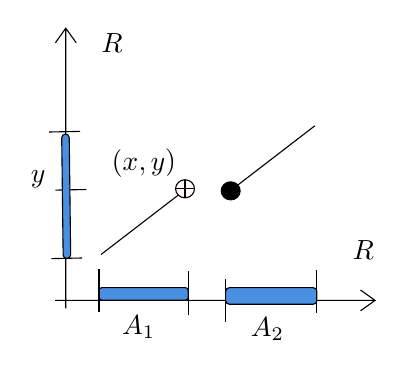
\begin{tikzpicture}[x=0.75pt,y=0.75pt,yscale=-1,xscale=1]
%uncomment if require: \path (0,300); %set diagram left start at 0, and has height of 300

%Shape: Axis 2D [id:dp26430596329710565] 
\draw  (49,214.44) -- (203.1,214.44)(54.1,83.3) -- (54.1,218.3) (196.1,209.44) -- (203.1,214.44) -- (196.1,219.44) (49.1,90.3) -- (54.1,83.3) -- (59.1,90.3)  ;
%Rounded Rect [id:dp051838128654554616] 
\draw  [fill={rgb, 255:red, 74; green, 144; blue, 226 }  ,fill opacity=1 ] (70.1,209.67) .. controls (70.1,208.91) and (70.71,208.3) .. (71.47,208.3) -- (111.74,208.3) .. controls (112.49,208.3) and (113.1,208.91) .. (113.1,209.67) -- (113.1,212.94) .. controls (113.1,213.69) and (112.49,214.3) .. (111.74,214.3) -- (71.47,214.3) .. controls (70.71,214.3) and (70.1,213.69) .. (70.1,212.94) -- cycle ;
%Rounded Rect [id:dp4090774294526508] 
\draw  [fill={rgb, 255:red, 74; green, 144; blue, 226 }  ,fill opacity=1 ] (131.1,210.12) .. controls (131.1,209.11) and (131.91,208.3) .. (132.92,208.3) -- (173.28,208.3) .. controls (174.29,208.3) and (175.1,209.11) .. (175.1,210.12) -- (175.1,214.48) .. controls (175.1,215.49) and (174.29,216.3) .. (173.28,216.3) -- (132.92,216.3) .. controls (131.91,216.3) and (131.1,215.49) .. (131.1,214.48) -- cycle ;
%Straight Lines [id:da64388132407526] 
\draw    (110.1,162.3) -- (71.1,192.3) ;
\draw  [fill={rgb, 255:red, 255; green, 250; blue, 250 }  ,fill opacity=1 ] (107,160.65) .. controls (107,158.25) and (109.04,156.3) .. (111.55,156.3) .. controls (114.06,156.3) and (116.1,158.25) .. (116.1,160.65) .. controls (116.1,163.05) and (114.06,165) .. (111.55,165) .. controls (109.04,165) and (107,163.05) .. (107,160.65) -- cycle ; \draw   (107,160.65) -- (116.1,160.65) ; \draw   (111.55,156.3) -- (111.55,165) ;
\draw  [fill={rgb, 255:red, 0; green, 0; blue, 0 }  ,fill opacity=1 ] (129,161.65) .. controls (129,159.25) and (131.04,157.3) .. (133.55,157.3) .. controls (136.06,157.3) and (138.1,159.25) .. (138.1,161.65) .. controls (138.1,164.05) and (136.06,166) .. (133.55,166) .. controls (131.04,166) and (129,164.05) .. (129,161.65) -- cycle ; \draw   (129,161.65) -- (138.1,161.65) ; \draw   (133.55,157.3) -- (133.55,166) ;
%Straight Lines [id:da6240534914484722] 
\draw    (174.1,130.3) -- (135.1,160.3) ;
%Straight Lines [id:da26345564387084763] 
\draw    (64,161) -- (49.1,161.3) ;
%Rounded Rect [id:dp5446725714009876] 
\draw  [fill={rgb, 255:red, 74; green, 144; blue, 226 }  ,fill opacity=1 ] (54.66,194.29) .. controls (53.66,194.31) and (52.84,193.5) .. (52.82,192.5) -- (52.13,136.12) .. controls (52.12,135.12) and (52.92,134.3) .. (53.92,134.29) -- (53.92,134.29) .. controls (54.92,134.28) and (55.74,135.08) .. (55.76,136.08) -- (56.44,192.46) .. controls (56.46,193.46) and (55.66,194.28) .. (54.66,194.29) -- cycle ;
%Straight Lines [id:da09701668858062606] 
\draw    (113.1,221.3) -- (113.1,200.3) ;
%Straight Lines [id:da006128268425505956] 
\draw    (70.1,220.17) -- (70.1,199.17) ;
%Straight Lines [id:da2642800457448089] 
\draw    (175.1,220.62) -- (175.1,199.62) ;
%Straight Lines [id:da346987503804841] 
\draw    (131.1,224.98) -- (131.1,203.98) ;
%Straight Lines [id:da3019826841878914] 
\draw    (61,133) -- (46.1,133.3) ;
%Straight Lines [id:da641826860041459] 
\draw    (62,194) -- (47.1,194.3) ;

% Text Node
\draw (80,220.4) node [anchor=north west][inner sep=0.75pt]    {$A_{1}$};
% Text Node
\draw (142,221.4) node [anchor=north west][inner sep=0.75pt]    {$A_{2}$};
% Text Node
\draw (70,84.4) node [anchor=north west][inner sep=0.75pt]    {$\mathbb{R}$};
% Text Node
\draw (191,184.4) node [anchor=north west][inner sep=0.75pt]    {$\mathbb{R}$};
% Text Node
\draw (74.85,140.59) node [anchor=north west][inner sep=0.75pt]  [rotate=-359.42,xslant=-0.01]  {$( x,y)$};
% Text Node
\draw (36,150.4) node [anchor=north west][inner sep=0.75pt]    {$y$};


\end{tikzpicture}

\begin{exercice}
    Quelle est la topologie induite sur $\mathcal C$ le tryadique de Cantor ?
\end{exercice}

\section{Sous-base de topologie}

\begin{definition}[Sous-base de topologie]
Soit $ \topologie$ une topologie et soit $S\subseteq\partie(X)$. On dit que $S$ est une sous-base de $\topologie$ si $S\subseteq \topologie$ et que pour toute topologie $\mathcal U$ sur $X$ étendant $S$, on a $\topologie\subseteq\mathcal U$.
\end{definition}
\begin{proposition}
    Soit $S\subseteq\partie(X)$. Alors il existe une et une seule topologie $\langle S\rangle$ telle que $S$ soit une sous-base de $\langle S\rangle$. De plus, $\langle S\rangle = \bigcap_{\topologie\in (S)}\topologie$ avec $(S)$ l'ensemble des topologies étendant $S$. On appelle $\langle S\rangle $ la topologie engendrée par $S$
\end{proposition}
\begin{proof} Montrons l'unicité, puis l'existence
\begin{description}
    \item[Unicité] Soit $\topologie_1,\topologie_2$ dont $S$ est une sous-base. Alors $\topologie_1,\topologie_2$ sont des topologies étendant $S$, donc $\topologie_1\subseteq\topologie_2$, et réciproquement.
    \item[Existence] Prenons $\langle S\rangle = \bigcap_{\topologie\in (S)}\topologie$. L'ensemble comprend $\partie(\partie(X))$ la topologie discrète donc l'intersection existe. Comme l'intersection de topologie est une topologie, $\langle S\rangle$ est une topologie. On a bien $S\subseteq\langle S\rangle$ car c'est l'intersection d'extension de $S$.
\end{description}
\end{proof}
\begin{proposition}On a
$\langle S\rangle=\langle S\cup\{\emptyset,X\}\rangle$
\end{proposition}
\begin{proof}
    Montrons que $\bigcap_{\topologie\in (S)}\topologie=\bigcap_{\topologie\in (S\cup\{\varnothing,X\})}\topologie$. Pour cela, il suffit de montrer que $(S)=(S\cup \{\varnothing,X\})$.
    \begin{description}
        \item[$(\subseteq)$:] Soit $\topologie\in (S)$ une topologie étendant $S$ (\textit{i.e} $S\subseteq \topologie$) Comme $\topologie$ est une topologie, par définition on a $\varnothing, X\in \topologie$ donc $S\cup\{\varnothing,X\}\subseteq \topologie$. C'est à dire que $\topologie\in (S\cup\{\varnothing,X\})$.
        \item[$(\supseteq)$ :] Soit $\topologie\in (S\cup\{\varnothing,X\})$ une topologie tel que $S\cup\{\varnothing,X\}\subseteq\topologie$. Puisque $S\subseteq S\cup\{\varnothing,X\}$, on obtient $\topologie\in (S)$.
    \end{description}
\end{proof}
\begin{proposition}
    Soit $S\subseteq\partie(X)$ tel que $\varnothing,X\in S$. Alors \begin{equation*}
        \langle S\rangle=\{A\subseteq X\mid A \text{ est union quelconque d'intersections finies d'éléments de } S\}=:\hat S
    \end{equation*}
\end{proposition}
\begin{proof}
 Démontrons l'égalité $\langle S \rangle = \widehat{S}$ par double inclusion.

\begin{description}
\item[ $(\subseteq)$] 
Il suffit de montrer que $\widehat{S}$ est une topologie contenant $S$.

D'abord, $S \subseteq \widehat{S}$ car tout $U \in S$ s'écrit comme intersection finie d'un seul élément.

Ensuite, $\widehat{S}$ est une topologie :
\begin{itemize}
\item $\emptyset, X \in S \subseteq \widehat{S}$ par hypothèse.
\item \textit{Union quelconque :} Si $A_i = \bigcup_{j \in J_i} (\bigcap_{k \in K_{i,j}} S_{i,j,k})$ avec $S_{i,j,k} \in S$, alors 
\[
\bigcup_{i \in I} A_i = \bigcup_{i \in I, j \in J_i} \left(\bigcap_{k \in K_{i,j}} S_{i,j,k}\right) \in \widehat{S}
\]
\item \textit{Intersection finie :} Pour $A = \bigcup_{j \in J} (\bigcap_{k \in K_j} S_{j,k})$ et $B = \bigcup_{\ell \in L} (\bigcap_{m \in M_\ell} T_{\ell,m})$, on a
\[
A \cap B = \left(\bigcup_{j \in J} (\bigcap_{k \in K_j} S_{j,k})\right)\cap\left(\bigcup_{\ell \in L} (\bigcap_{m \in M_\ell} T_{\ell,m})\right)=\bigcup_{j \in J, \ell \in L} \left(\bigcap_{k \in K_j} S_{j,k} \cap \bigcap_{m \in M_\ell} T_{\ell,m}\right) \]
Comme on l'a démontré dans la section sur les familles.
\end{itemize}
\smallskip
Donc $\widehat{S}$ est une topologie contenant $S$, d'où $\langle S \rangle \subseteq \widehat{S}$.

\medskip
\item[$(\supseteq)$] 
Soit $A \in \widehat{S}$, alors $A = \bigcup_{i \in I} (\bigcap_{j \in J_i} S_{i,j})$ avec $S_{i,j} \in S$.

Puisque $\langle S \rangle$ est une topologie contenant $S$, elle est stable par intersections finies et unions quelconques. Donc $A \in \langle S \rangle$.
\end{description}
\end{proof}
\begin{definition}[Base de topologie]
Soient $S\subseteq\partie(X)$ et $\topologie$ une topologie sur $X$. On dit que $S$ est une base de $\topologie$ si $$
\forall\ouvert\in\topologie,\ouvert = \bigcup_{i\in I}S_i\text{ avec $(S_i)_{i\in I}$ une famille d'éléments de $S$}$$
\end{definition}
\begin{proposition}
    Soient $S\subseteq\partie(X)$ et $\topologie$ une topologie sur $X$. $S$ est une base de $\topologie$ ssi
    \begin{itemize}
        \item $\topologie=\langle S\rangle$
        \item $\bigcup_{A\in S}A= X$
        \item Toute intersection finie d'éléments de $S$ peut s'écrire comme une union quelconque d'éléments de $S$
    \end{itemize}
\end{proposition}
\begin{proof}
    Flemme
\end{proof}
\section{Topologie métrique}
\begin{definition}[Distance]
    Soit $E$ un ensemble, une distance $d$ est une fonction de $E\times E$ dans $[0,+\infty[$ vérifiant :
    \begin{enumerate}
        \item $\forall x,y\in E,\ d(x,y)=0 \Leftrightarrow x=y$
        \item $\forall x,y\in E,\ d(x,y)=d(y,x)$
        \item $\forall x,y,z \in E,\ d(x,y)\leq d(x,z)+d(z,y)$
    \end{enumerate}
\end{definition}
\begin{exemple}
Sur $\mathbb{R}$, l'application $d(x,y)=|x-y|$ est une distance. Sur $E$ un ensemble non vide, on peut définir la distance discrète :
\begin{equation*}
    d(x,y)=\begin{cases}
1 & \text{si } x \neq y, \\
0 & \text{si } x = y.
\end{cases}
\end{equation*}
\end{exemple}
\begin{definition}
    Soit $x\in X, \varnothing\ne A\subseteq X$. On définit la distance $d(x,A)$ par $d(x,A) = \inf\limits_{y\in A}d(x,y)$.
    Comme $\{d(x,y)\mid y \in A\}\subseteq\R^{\ge0}$ est non vide, donc l'infimum existe.
\end{definition}
\begin{remarque}
    $d$ est continue.
\end{remarque}
\begin{definition}[Norme]
    Soit $E$ un $\mathbb{K}-$espace vectoriel. Une norme $\norm{\cdot}$ est une application de $E$ dans $[0,+\infty[$ qui vérifie:
    \begin{enumerate}
        \item $\forall x\in E,\ \norm{x}=0 \Rightarrow x=0$
        \item $\forall\lambda\in \mathbb{K},\ \forall x\in E,\ \norm{\lambda x}=|\lambda|\norm{x}$
        \item $\forall x,y\in E,\ \norm{x+y}\leq \norm{x}+\norm{y}$
    \end{enumerate}
\end{definition}
\begin{definition}
    Soient $E$ un $\mathbb{K}$-espace vectoriel et une norme $\norm{\cdot}$. On dit que le couple $(E,\norm{\cdot})$ est un espace vectoriel normé (EVN).
\end{definition}
\begin{exemple} 
Voyons quelques exemples d'EVN.
    \begin{itemize}
        \item $(\R,\abs{\cdot})$ est un EVN.
        \item $(\C,\abs{\cdot})$ est un EVN.
        \item Sur $\R^n$ (ou $\C^n$) on peut définir les normes suivantes :
        \begin{enumerate}
            \item $\norm{x}_1=\sum_{i=1}^n|x_i|$
            \item $\norm{x}_2=\sqrt{\sum_{i=1}^n|x_i|^2}$
            \item Soit $p>1$, $\norm{x}_=\left(\sum_{i=1}^n|x_i|^p\right)^{\frac 1 p}$
            \item $\norm{x}_\infty=\max_{1\leq i\leq n}|x_i|$
        \end{enumerate}
    \end{itemize}
\end{exemple}
\begin{remarque}
    Une norme $\norm{\cdot}$ induit une distance $d$ définie par $d(x,y) = \norm{x-y}$
\end{remarque}
\begin{definition}[Boule ouverte]
   Soit $(X,d)$ un espace métrique, $\textit{i.e.}$ $d$ est une distance sur $X$. La boule ouverte centrée en $a\in X$ de rayon $r>0$ est définie par $B(a,r):=\{x\in X\mid d(x,a)<r\}$
\end{definition}
\begin{definition}
    Soit $(X,d)$ un espace métrique. La topologie sur $X$ associée à $d$ est la topologie engendrée par les boules ouvertes pour la distance $d$.
\end{definition}
\begin{proposition}
    Soit $\R^2$ avec la distance $d_2$. Soit $S$ l'ensemble des boules ouvertes pour $d_2$
    Soit $c_1,c_2\in \R^2$ $r_1r_2\in \R^{>0}$ Soient $B_1=B(c_1,r_1)$ et $B_2=B(c_2,r_2)$ Soit $x_0\in B_1\cap B_2$, donner explicitement en fonction de la position de $x_0$ une boule ouverte de rayon $\varepsilon$ telle que $B(x_0,\varepsilon)\subseteq B_1\cap B_2$
\end{proposition}
\begin{proof}
    Prenons $\varepsilon :=\min\{r_1-d_2(c_1,x_0),r_2-d_2(c_2,x_0)\}>0$. Et montrons que $B(x_0,\varepsilon)\subseteq B_1\cap B_2$. Soit $x\in B(x_0,\varepsilon)$. Montrons que $x\in B_1\cap B_2$.
    \begin{description}
        \item[$(x\in B_1)$ :] On a les inégalités suivantes :
        \[
         d_2(c_1,x)\leq d_2(c_1,x_0)+d_2(x_0,x) < d_2(c_1,x_0)+\varepsilon\leq  d_2 (c_1,x_0)+r_1 -d_2(c_1,x_0)=r_1
        \]
        \item[$(x\in B_2)$ :] On utilise le même raisonnement qu'au point précédent.
    \end{description}
\end{proof}
 on en conclut que $B_1\cap B_2=\bigcup_{x\in B_1\cap B_2}B(x,\varepsilon_x)$ et donc, on a que les intersections finies de boules ouvertes sont des unions quelconques de boules ouvertes et donc les boules forment une base de topologie. La topologie engendrée par les boules est dite associée à la norme $\norm{\cdot}_2$ est notée $\topologie_2$. Idem pour $\topologie_1,\ \topologie_\infty$.
 \section{Densité}
Soit $(X,\topologie)$ un espace topologique, on dit que $Y$ est ($\topologie-$)dense dans $X$ si pour tout $\ouvert\in \topologie,\ \ouvert\cap Y\neq \varnothing$,  (ce qui est équivalent, en acceptant l'axiome du choix, à  pour tout $\ouvert\in\topologie$, il existe $y_o\in \ouvert\cap Y$). De façon équivalente, on peut dire $Y$ est dense dans $X$ ssi pour tout voisinage $V$, il existe $y\in V\cap Y$.Si $\topologie$ admet une base $S$ alors c'est équivalent à ce que $\forall B\in S,\ B\cap Y\ne\varnothing$. 
\begin{exemple}
    $\mathbb{Q}$ est $\topologie_2-$dense dans $\R$. On utilise le fait que tout ouvert est une union de boules ouvertes; donc  il suffit de prouver que si
    $B(x,r)$ est une boule ouverte, j'y trouve un rationnel. Ici $B(x,r)=]x-r,x+r[$, il faut trouver $q\in ]x-r,x+r[$ Comment placer un rationnel $r-$proche de $x$ ? Si on admet que les réels sont des limites de suites de Cauchy de rationnels, on prend une telle suite $q_n$ convergeant vers $x$ et on sait qu'il existe $n_0$ tel que pour tout $n\geq n_0\quad |q_n-x|\leq \frac{r}{2}$
   Considérons l'écriture décimale de $x$, càd prenons $z\in\Z,\forall i\in\N_0, d_i\in\{0,1,\ldots,9\}$ tels que $x=\overline{ z,d_1d_2...d_k...}_{10}$ ou autrement dit $x=z+\sum_{i=1}^\infty d_i10^{-i}$
    Et clairement $x_k=z+\sum_{i=1}^kd_i10^{-i}$ vérifie que 
    \[
    |x-x_k|=\sum_{i=k+1}^\infty d_i10^{-i}\leq g\sum_{i=k+1}^\infty10^{-i}=g\cdot10^{-(k+1)}\sum_{i=0}^\infty10^{-i}=g\cdot10^{-(k+1)}\frac{1}{1-\frac{1}{10}}=10^{-k}
    \]
    On cherche $q\in ]x-r,x+r[$. On peut pour cela prendre $x_k$ tel que $|x-x_k|\leq \frac{r}{2}$ càd tel que $10^{-k}\leq \frac{r}{2}$.
\end{exemple}
\begin{remarque}
    Tout cela est possible car $\R$ est un groupe archimédien (dont l'ordre est en plus compatible avec $\cdot$)
    \[
    \R^{\geq0}=\bigsqcup_{n\in \N}[n,n+1[
    \]
\end{remarque}
\begin{definition}
    Un groupe ordonné $(G,+,\leq)$ est dit archimédien si $\leq$ est total, compatible avec plus et tel que $\forall a\in G^{>0},\forall b\in G^{\geq 0},\ \exists n\in\N, an\geq b$
\end{definition}


\begin{proposition}
        Soit une boule ouverte $B(x,r)$ non vide de $\R^2$, alors $B(x,r)\cap \Q^2\neq \emptyset$. 
\end{proposition}

\begin{proof}
on a que $x=(x_1,x_2)$ où $x_1,x_2\in \R$. Par définition de $\R$. Il existe $(q_{1_n})_{n\in I}\subseteq \Q$ et $(q_{2_n})_{ n\in J }\subseteq \Q$ convergeant respectivement vers $x_1$ et $x_2$. On considère donc la suite $(q_n)_{n\in I\cap J}\subseteq \Q^2$ où $q_n=(q_{1_n},q_{2_n})$. Puisque la convergence des suites dans $\R^n$ revient à la convergence coordonnée par coordonnée. On a donc trouvé une suite $(q_n)\subseteq \Q^2$ convergeant vers $x\in\R$. Nous avons donc :
\begin{equation*}
    \forall\varepsilon>0, \exists n_0\in I\cap J, \forall n\geq n_0 \quad \norm{q_n-x}<\varepsilon
\end{equation*}
On utilise l'équation avec $\varepsilon=r$, il existe donc $n_0\in I\cap J$ tel que $\norm{q_{n_0}-x}< r$. On a donc $q_{n_0}\in B(x,r)\cap \Q^2$. Autrement dit, on vient de montrer que 
\[
B(x,r)\cap \Q^2\neq \varnothing
\]
\end{proof}

Avec ce résultat, prouvons que l'intersection de $2$ boules ouvertes de $\R^2$ est une union dénombrable de boules ouvertes.
\[
B_1\cap B_2\neq \emptyset
\]
On considère
$\mathbb{Q}^2\cap (B_1\cap B_2)\neq \emptyset$
En fait, il existe $S$ dénombrable tel que $\topologie_2=(S)$. \begin{proposition}
    Toute $B(x,r)$ est une union dénombrable de $B\left(x, \frac{1}{n}\right)$ avec $x\in \mathbb{Q}^2 $
\end{proposition}
\begin{proof}
    Montrons que $B(x,r)= \bigcup_{(q,\varepsilon)\in Q}B(q,\varepsilon)$ avec $Q:=\{(q,\varepsilon)\in\Q^2\times \Q\mid \exists n\in\N,\ \varepsilon=\frac 1 n ,\ B(q,\varepsilon)\subseteq B(x,r)\}$.
    \begin{description}
        \item[$\supseteq$ : ]Trivial car tous les éléments de l'union sont $\subseteq B(x,r)$
        \item[$\subseteq$ : ]Soit $y\in B(x,r)$. Comme $r':= r-d(y,x)>0$, il existe par le point précédent $q_y\in \Q^2,\varepsilon_y\in\{\frac 1 n\mid n\in\N\}$ tels que $B(q_y,\varepsilon_y)\subseteq B(y,r')$. Soit $z\in B(y,r')$. On a $d(z,r)\leq d(y,z)+d(y,x)<r-d(y,x)+d(y,x) = r$ d'où $B(q_y,\varepsilon_y)\subseteq B(y,r')\subseteq B(x,r)$ et donc $y\in B(q_y,\varepsilon_y)\subseteq \bigcup_{(q,\varepsilon)\in Q}B(q,\varepsilon)$
    \end{description}
\end{proof}